\documentclass{report}

\usepackage{graphicx}

%left margin gutter
\oddsidemargin 0.0in
%right margin gutter
\evensidemargin 1.0in
\textwidth 6.5in
%distance from bottom of top margin to top of writing
\headheight 0.0in
\topmargin 0.0in
\textheight 8.5in

%title info
\title{{\LARGE {\bf Interim Report\\}}YardSale\\The Open Source Point of Sale Solution}
\author{Jesse Lovelace\\Adam Parrish\\Mike Swigon\\Jay Johnston\\John Lamb\\Cameron Watts}
\date{March 5, 2004}

\begin{document}

\maketitle

\tableofcontents

\chapter{Requirements Definition}

\section{Introduction}

YardSale is an open source Point of Sale system that is being
designed by A.S Logic Systems to revolutionize the way Point of
Sale systems are implemented in today's market.  Current
implementations of Point of Sale systems are fraught with a number
of issues; including often being extremely overpriced, difficult
to administer, dated in their functionality, and lacking necessary
operations.  YardSale was designed to alleviate these problems and
allow for extensibility as the market of retail sale expands in
the future.

Being that YardSale is an open source project with little funding,
the initial niche market will target small, locally owned retail
stores.  This type of market will allow for extensive on-site
research, as many of these businesses should be willing to work
with us to improve on the functionality of their existing POS
system.  In addition, because A.S. Logic has decided to take the
open source route, the software itself will be freely available to
all who wish to use it, the only expense that will come into play
is if the company wishes to enlist our services in setup,
troubleshooting, support, expansion, or customization.

\section{Functional Requirements}

This section entails all of the minimal requirements set by the AS
Logic Systems development team for the OpenPOS hereafter referred
to as YardSale.\\
\\Minimum functionality of YardSale should accomplish the
following:

\begin{itemize}
    \item {Manage Inventory Data}
    \item {Manage Customer Data}
    \item {Manage Employee Data}
    \item {Perform Transactions}
    \item {Provide Logging Facilities}
    \item {Report on Data}
    \item {User Level Access Rights}
\end{itemize}

Each of these tasks is described in depth in their corresponding
sub sections. There is planned functionality above and beyond this
basic featureset, although without these functions other
functionality can not be added.

    \subsection{Database Management}
    The goal of the database management tasks are to add, modify, and
    delete information in the database. The database backend will run
    on a MySQL server and all relevant data will be stored in its own
    table or set of tables. More information on the database design
    can be found in the database design document.

    \subsubsection{Inventory Management}
    The inventory management system will have an interface for the
    stock employees to enter new shipments. It will also have an
    interface for the management employees to define new items for
    sale. The most common use of the inventory management system will
    be integrated into the checkout system. When customers are
    checking out, inventory will be populated to the checkout screen
    from the database, and then decremented on purchase from their
    quantity in the database.

    \subsubsection{Customer Management}
    The customer management system will work in a similar fashion to
    the inventory management system. It will have only one level of
    functionality though, the ability to define and update new
    customer data. There will also be a small interface with the
    database during the checkout of a customer which will allow for
    the selection of a customer from the customer table.

    \subsubsection{Employee Management}
    The employee management system here again will also function
    similarly to the previous two in that it has hooks into the
    database for employees. It will allow an authorized user the
    ability to add and modify employee information as well as
    disable employee accounts.\\
    \\

    {\sl Among the more specific functionality of each of these sections
    will be to allow the user to retrieve any item stored in either
    inventory, customer, or employee tables given a search
    criteria.}

    \subsection{Transactions}

    Transactions in YardSale are basically a 4 step process. The first
    step in the process is to select a customer to do business with or
    select a cash "quick" customer. After the customer is selected
    their basic information will be displayed on the main checkout
    screen. The user will will then either select items from the
    inventory from a hierarchy, scan them in with the barcode scanner,
    or manually type in their information in lookup fields to checkout
    a customer. A running total will be kept as well as tax
    calculations for the sale. After all items are accounted for a
    checkout screen will be called. This will allow the user to select
    the customer's preferred method of payment and also provide the
    user with the ability to calculate the correct amount of change.

    All transactions will be maintained with a table in the database
    that will link related elements of the transaction together for
    later reporting.

    \subsection{Logging}
    Many program logging features will be provided inherently due to
    the database backend. Among the logging facilities will be the
    following items:

    \begin{itemize}
        \item {Employee Time Tracking}
        \item {Transaction Logging}
        \item {Shipment Logs}
        \item {SQL String Execution Logging}
    \end{itemize}

    Employee time tracking will be logged based on when the login to
    their first client and when the logout of their last client. An
    entry in the Login table will track this for each instance of a
    session. The transaction logging as was discussed earlier will be
    maintained in a table of its own tracking related items,
    customers, and employees with transactions. The shipment logs will
    be an offshoot of a transaction in that some will be shipped. If
    so a log of the shipping information will be available as it
    relates to the customer and the carrier. As a debugging feature a
    SQL String Execution Log facility will also be included. For every
    SQL string used on the database, there will be a stored procedure
    that adds it to the log table for later searching and debug use.
    This feature will likely be disabled in the final deliverable.

    \subsection{Reporting}
    There will be a wide variety of reporting features available also
    as a result of the database backend. The following basic reporting
    functionality will be available in the first iteration of
    YardSale.

    \begin{itemize}
        \item{Payroll for Employees}
        \item{Top Sales for Inventory Items}
        \item{Top Sales for Employees}
        \item{Top Sales for Customer}
        \item{Revenue Reporting given any time frame}
        \item{Hourly Employee Log Reporting}
    \end{itemize}

    All of the reports will be output to a pdf via \LaTeX type
    setting. This will provide ease of portability and a wide range of
    flexibility in reporting.

    \subsection{User Level Access Rights}
    YardSale has three different levels of user interactivity. There
    are Managers, Sales Associates, and Administrative users.

    \subsubsection{Sales Associate Functionality}
    Sales associates are likely going to be the primary users of the
    YardSale system. However they will have a limited set of
    functionality when they login. Their privileges will be limited to
    basic customer management and transaction processing. They have no
    real need for full inventory capabilities nor do they need the
    ability to manage or browse employee information.

    When a sales associate logs into YardSale they will see the following options:

    \begin{itemize}
        \item Transaction Processing
        \item Customer Management
    \end{itemize}

    \subsubsection{Manager Functionality}
    The managers primary function in YardSale is to make sure that all
    of the inventory items, customers, and employees are correctly
    maintained. They are also the only primary user on the system
    allowed to run reporting functions.

    When a manager logs in to YardSale they will have a full set of
    functionality available to them from the main screen inclusive of
    the following:

    \begin{itemize}
        \item Inventory Management
        \item Transaction Processing
        \item Customer Management
        \item Employee Management
        \item Reporting
    \end{itemize}

    \subsubsection{Administrative Functionality}

    The administrative user is basically a built in manager user. This
    user will have full rights to the system and the password will be
    able to unlock other accounts in the system that are locked due to
    loss of password. The administrative user will likely never be
    used in day to day use of YardSale, however it is provided as a
    safety to always allow the access of encrypted data in case of
    total loss of management capability.

\section{Non Functional Requirements}

    \subsection{Cross Platform}
    The YardSale software is to be developed using the wxWindows libraries for C++,
    which creates GUIs (Graphical User Interfaces) that are
    platform independent.  The YardSale software will be able to
    run on any major operating system on today's market.

    \subsection{Cross Architecture}
    The main purpose of the YardSale software is to be very
    independent of all architectural aspects of the system, using
    minimal system resources.  The idea is to be able to use any system
    to run the software appropriately.

\section{External Dependencies and Interfaces}

    \subsubsection{Cash Drawers}
    The cash drawers used for the system are a serial interface,
    which must be supported by each client system.  The drawers
    must open automatically when a transaction is completed; and
    manually by managers and authorized users.

    \subsubsection{Magnetic Card Scanners}
    The magnetic card scanners serve multiple purposes, but all with
    similar functionality.  The scanners are a serial interface,
    which must be supported by each client system.  They must read the
    information stored on the card and relay it to the system.
    The system will use this interface for both credit card
    transactions and user access.

    \subsubsection{Barcode Scanners}
    The barcode scanners are a USB (Universal Serial Bus)
    interface, which must be supported by each client system.  They must
    read the barcode scanned and relay the information about the
    product to the system.

    \subsubsection{Receipt Printers}
    The receipt printers are a printer (parallel) interface, which
    must be supported by each client system.  The printers
    will print specified information at the conclusion of each
    transaction; and will also be able to print daily user reports.

    \subsubsection{TouchScreen Monitor}
    Touch screen monitors will be used at every sales location.
    The monitors use a USB interface, which must be supported by
    each client system.  The touch screens will act as both the
    monitor and mouse of the system for easy accessability.  The
    monitors must correctly read the commands given and relay them
    to the system.

\section{Preliminary Design}

    \subsection{Major Modules}

        \subsubsection{YardDatabase}
        The YardDatabase module works as the translator between
        the user interface and the database.  It converts calls
        made by the GUI into SQL queries to be sent to the
        database.  When the query results are returned from the
        database, YardDatabase converts these items to a
        YardDBType (discussed in next section) to be read by the
        GUI.
        \subsubsection{YardDBType}
        The YardDBType module is the superclass for all information that
        may be sent to the GUI from the database.  It contains
        function calls for each of the following types:
        \begin{list}{}
            \item{{\bf YardInvType:} contains variables for all
            possible inventory management items stored in the
            database.  Coordinates with the Inventory Management
            view in the GUI, which is also used by Transactions.}
            \item{{\bf YardCustomerType:} contains variables for
            all possible customer management items stored in the database.
            Coordinates with the Customer view in the GUI,
            which is also used by Transactions.}
            \item{{\bf YardEmployeeType} contains variables for
            all possible employee management items stored in the
            database.  Coordinates with the Employee Management
            view in the GUI.}
            \item{{\bf YardTransaction} contains variables for all
            possible transaction items stored in the database.
            Coordinates with the Transaction view in the GUI.}
        \end{list}{}
        \subsubsection{GUI wxWidges}
        The wxWidges module defines all interfaces used by the
        GUI.  It contains functions derived from the wxWindows
        libraries for C++.  It also interacts with the
        YardDatabase module to display information sent from the
        database.


    \subsection{System Architecture}
    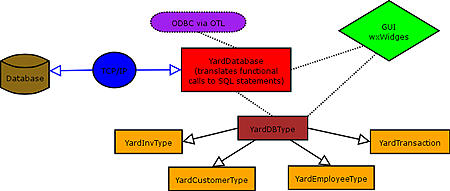
\includegraphics{yardsale_modules.png}

\section{Preliminary Project Task Plan}
    %Scope and Size of Project Paragraph

    \subsection{Milestones}
    \begin{description}
        \item[2004-03-05] FEATURE FREEZE - deadline for adding functional
        features to the design of the POS.
        \item[2004-03-07] ITERATION 1 - all requirements for first
        iteration to be completed and documented in the interim
        report.
        \item[2004-04-01] ITERATION 2 - all secondary requirements
        to be completed for the second iteration.
        \item[2004-04-17] CODE FREEZE - deadline for beginning the
        coding of features; those not already implemented will be removed;
        testing only beyond this point
        \item[2004-04-27] FINAL DELIVERABLE - completion of
        prototype for presentation to the CSC department at the
        Posters and Pies event.
    \end{description}

    \subsection{Team Member Roles and Responsibilities}

    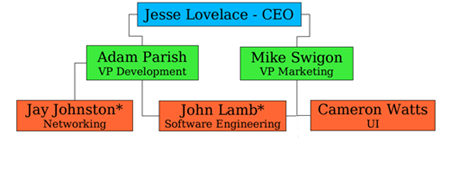
\includegraphics{organization.png}
    \\The team roles are defined as follows:

    \begin{description}
        \item[Jesse Lovelace] As the CEO of A.S. Logic Systems,
        Jesse is in charge of all aspects of the project.  Though
        he works very closely with both VPs, Jesse is the ultimate
        decision maker for the team.  In addition to his roles as
        CEO, Jesse is also in charge of the design and
        implementation of the User Interface and all security
        aspects.
        \item[Adam Parrish] Adam is the Vice President in charge
        of Development at A.S Logic Systems.  He works closely
        with both the CEO and VP of Marketing to see that
        YardSale's implementation is both correct and timely.  In
        addition to these company roles, Adam is also the lead
        Database Programmer; seeing to it that the database is
        functioning properly and creating the SQL scripts for
        populating and querying the database.
        \item[Mike Swigon] Mike is the Vice President of
        Marketing at A.S. Logic Systems.  He works closely with
        both Adam and Jesse to both design the entire system and
        to insure that its implementation is correct.  In addition
        to these responsibilities, Mike works with Adam in database
        setup and creation of SQL scripts for populating and
        querying the database.
        \item[John Lamb] John's responsibilities fall primarily in
        interfacing with the database.  He works closely with Jesse
        to develop a UI that can correctly and securely
        communicate information to and from the database; also
        implementing the SQL statements developed by Mike and
        Adam.
        \item[Jay Johnston] Jay's responsibilities fall primarily
        in creation of the UI and networking the system during
        setup.  He works closely with Jesse to develop modules
        for required functionality of the interface.
        \item[Cameron Watts] Cameron's responsibilities fall
        primarily on marketing and system research.  He works
        closely with the design group to ensure YardSale's
        functionality is top-of-the-line and user friendly.
    \end{description}


\chapter{Design}

	The following sections are related to the design of YardSale
	in regards to the database level design as well as the client
	application level design. The first section provides a high level
	explanation of the database architecture using UML diagrams. The
	following section explains design related issues of the YardSale
	client program.

\section{YardSale Database Design}

	The YardSale database was designed with security and efficiency in
	mind. The goal was, as it is in any database, to seperate unrelated
	data and key similar items together with table relations. The global
	database model is seen in the diagram on the following page. Although
	it is not necessarily easy to read the table relations can be seen, and
	table specifics like field values, indexes, and foreign and primary keys
	can be seen in the following table diagrams.

	\newpage

	\bf{YardSale Global Database Diagram}\\
	\\
	\\
	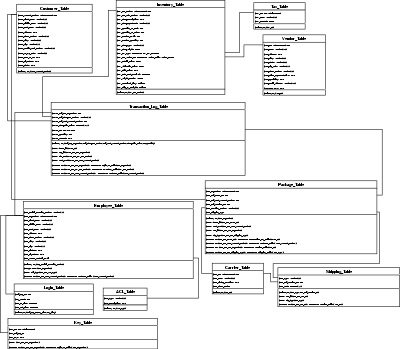
\includegraphics{Database_Layout.png}

	\newpage

	\subsection{Customer Management}

	Since customer management is basically a simple task it is maintained in only
	one table. There is no real need to have their data stored accross many
	different tables since all of the information is just personal data.

	\bf{Customer Table}\\
	\\
	\\
	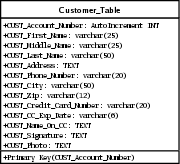
\includegraphics{Tables/CustomerTable.png}\\
	\\
	The above UML diagram shows the layout of the customer table. The object of this
	table is to manage customer personal information for later reference in
	transactions. By allowing this associativity YardSale will later be able to
	formulate reports on how much each of its customers spend for example. It also
	provides a rather in depth directory of all of a business's clients for use
	in any form they see fit.

	The data stored begins with the customer account number which is just an
	arbitrarily assigned number that is managed by the database management
	system. It is also the primary key for the table and is therefore unique.
	First, Middle, and Last names are all stored in seperate fields of their own,
	as is the Address information. Credit information can also be stored about users
	but is optional, and is also planned to be stored in the field as an encrypted
	string of data so that underprivileged users can not access it. Two interesting
	features about this table is the ability to store a link to a photograph and
	signature for each customer. That way it will aid in positively identifying a
	customer when they are checking out with check or credit.


	\newpage

	\subsection{Inventory Management}

	YardSale's Inventory Management scheme spans over three tables. The main table that
	stores actual inventory description information is the Inventory Table itself. The
	other two tables are used to support the main table. They are the Tax table and the
	Vendor Table. The tax table is basically a storage area for different tax types, and
	the Vendor Table is a storage table for Vendor information or Inventory Supplier
	information.\\
	\\
	\bf{Inventory Table}\\
	\\
	\\
	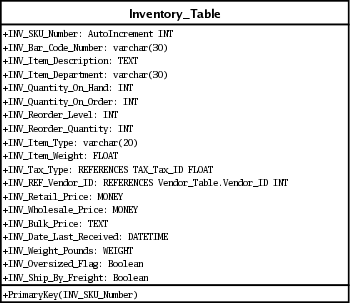
\includegraphics{Tables/InventoryTable.png}\\
	\\
	\\
	This table being the main Inventory storage structure contains all information needed
	about any inventory item. The record primary key is the SKU number which is a user
	defined number or character string. These are often used in small businesses to
	internally key their inventory. Manufacturers will often have a bar code associated
	with each item the produce as well so their is a field available for that as well.
	Each item can be briefly described, and associated with a department for further
	subcatagorizing. The number of any particular item is maintained as well as how many
	of the item are on order. There is a field for storing the number at which an item should
	be reordered, and also how many to reorder at that time. There are varying description
	fields such as item type and weight as well. Three pricing fields are supplied. The
	first two are statically maintained as retail and wholesale price. The third price
	type varies on the number of items being purchased. This field is maintained in XML
	format so that as many different pricing levels as are needed can be defined. When an
	item is received it updates the field corresponding to last received. Some items are
	oddly shaped or are overly heavy, either of these two options could cause the oversized
	flag to be set, and if the oversized flag is set a ship by freight option would also be
	set, but they are mutually exclusive and the ship by freight can be set without the
	oversized flag being set.\\
	\\
	\bf{Tax Table}\\
	\\
	\\
	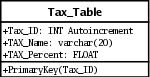
\includegraphics{Tables/TaxTable.png}\\
	\\
	\\
	The tax table is just a support table for the inventory items. It is referenced by ID
	depending on the desired taxing an item should have. Using a table allows for user definable
	tax types, and allows the database to be flexible to tax changes. All that the table needs
	is a Tax Name and a percentage for taxing items. The ID field is managed internally by the
	database management system and is also the primary key for the table.\\
	\\
	\bf{Vendor Table}\\
	\\
	\\
	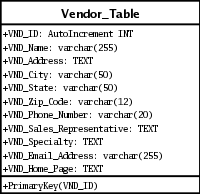
\includegraphics{Tables/VendorTable.png}\\
	\\
	\\
	The Vendor Table is used also as a supporting table for the inventory. This information
	pertains to the supplier of the items being sold. When an item reaches its reorder level
	in the Inventory Table, the information in this table would be used to make the order to
	resupply. The table is keyed by a unique ID that is managed by the database management
	system. The company name, address, and pertinent contact information is maintained along
	with a sales representative's name. There are optional fields for company specialty, email
	address, and homepage as well.

	\subsection{Transaction Handling}

	Transaction Handling is a process that has data spanning two tables with two more supporting
	tables. Transaction handling is split into two sections. The first section being the actual
	day to day transaction, and then the added functionality of packaging the items sold during
	the transaction.\\
	\\
	\\
	\bf{Transaction Table}\\
	\\
	\\
	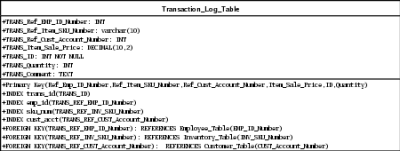
\includegraphics{Tables/TransactionLogTable.png}\\
	\\
	\\
	The Transaction Log Table is used to store information that links Customers, Employees, and
	inventory items. Each entry in the transaction table represents an item sold during a transaction.
	Since the key is not a single ID number it is the combination of the Customer, Employee, Item,
	Quantity and Price, the ID can be used to represent the overall transaction. Any row that contains
	an equivalent ID belongs to the same transaction.
	\\
	\\
	\bf{Package Table}\\
	\\
	\\
	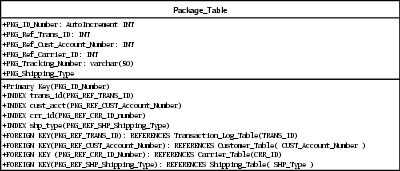
\includegraphics{Tables/PackageTable.png}\\
	\\
	\\
	The Package Table is used to store information about a package. There is a link to a transaction ID
	so that items can be associated with a package. There is also a link to a customer from the package
	table. The reason there is a link from the package table is because one customer may wish to buy
	something for another so the customer who made the transaction will not necessarily be the same as
	the one who will receive the package. There is also a reference to a carrier and a shipping type.
	A tracking number field is provided for when the tracking number is issued by the Carrier.
	\\
	\\
	\bf{Carrier Table}\\
	\\
	\\
	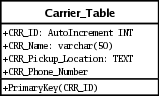
\includegraphics{Tables/CarrierTable.png}\\
	\\
	\\
	The Carrier table is a support table for the Package table. It provides information about the different
	shipping services. The information maintained here is just what is necessary to get a package shipped.
	There is a phone number, pickup location and an ID associated with each entry.
	\\
	\\
	\bf{Shipping Table}\\
	\\
	\\
	The Shipping Table is also a support table for the Package Table. This table is a list of all of the
	different methods of shipping available associated with the Carrier Table. Since each Carrier can
	have multiple shipping methods they can all be easily added and deleted if they ever change via
	this table. The table just contains the name for the type of shipping, the carrier, and how much
	it costs.\\
	\\
	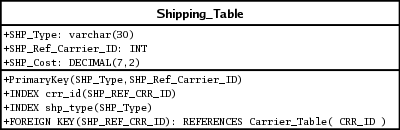
\includegraphics{Tables/ShippingTable.png}\\
	\\
	\subsection{Employee Management}

	The Employee Management section is actually two sections. There is the Employee portion which
	spans two tables, the Employee Table for employee information, and the Login Table which
	keeps track of the hours an employee works between logging in and out of the clients. The
	other section is the security aspect of the program as it relates to employees. It also spans
	two tables; the ACL Table and the Key Table.\\
	\\
	\bf{Employee Table}\\
	\\
	\\
	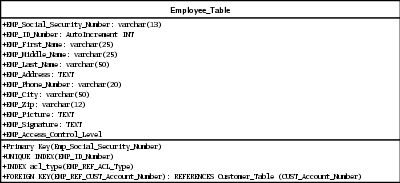
\includegraphics{Tables/EmployeeTable.png}
	\\
	\\
	The Employee Table keeps track of all pertinent information about employees that would
	be needed by an employer. Basic personal information such as First, Middle, and Last name
	as well as Contact information are maintained here. Each employee in the table has a unique
	employee identification number associated with them to avoid having to use the Social
	Security Number as a key. This also allows data such as the Social Security number to be
	encrypted to alleviate underprivileged users from seeing it. Each employee also has a
	field for a picture link and signature link to help with positive identification. The other
	field in this table is the password field which is used to store a users password to allow
	a user to login, and which is also used to decrypt the keys from the key table. Each user
	is also associated with a ACL entry in the ACL Table.\\
	\\
	\bf{Login Table}\\
	\\
	\\
	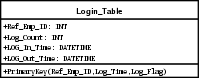
\includegraphics{Tables/LoginTable.png}\\
	\\
	\\
	The Login Table tracks the amount of time an employee has been logged in based on when
	they logged into their first client to when they logout of their last client. The structure
	is very simple. It references an employee ID and has a Count field. When the count is greater
	than zero the user is logged in and upon first entry a value will be inserted into the
	Log In Time field. When the value of Count reaches zero again a value will be inserted into
	the Log Out Time field.
	
	\subsubsection{Security}

	\bf{Access Control List Table}\\
	\\
	\\
	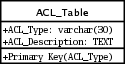
\includegraphics{Tables/ACL.png}\\
	\\
	\\
	The ACL table which is short for Access Control List Table manages which user types have access
	to different levels of program use. All this table contains is a Name of a user type and a description
	of their functionality. Currently we foresee only four user types and will likely not have an
	interface to manage this table.\\
	\\
	\\
	\bf{Key Table}\\
	\\
	\\
	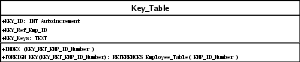
\includegraphics{Tables/KeyTable.png}\\
	\\
	\\
	The Key Table is used to manage the keys used to unencrypt the data stored in the database. The
	entry in this table will reference a valid user in the Employee Table and the text field will
	contain encrypted data that the user's password was used to encrypt. When the password is used
	to decrypt this data the user can obtain the keys used to encrypt global database data. A few
	example fields that are going to be stored as encrypted data are Credit Card Numbers and Expiration
	Date pairs as well as Social Security Numbers. This will add a level of database security that
	will prevent or deter malicious users from stealing valuable information from the database.\\
	\\

	\newpage
	
	\section{YardSale Client Application Design}

\chapter{Implementation}

	\subsection{Class Documentation}

Please note the following section was auto-generated. We are
working on tweaking this output a little, but currently it is
sectioned wrong.

%\section{Yard\-Database Class Reference}
\label{classYardDatabase}\index{YardDatabase@{YardDatabase}}
{\tt \#include $<$ys\_\-database.h$>$}

Collaboration diagram for Yard\-Database:\begin{figure}[H]
\begin{center}
\leavevmode
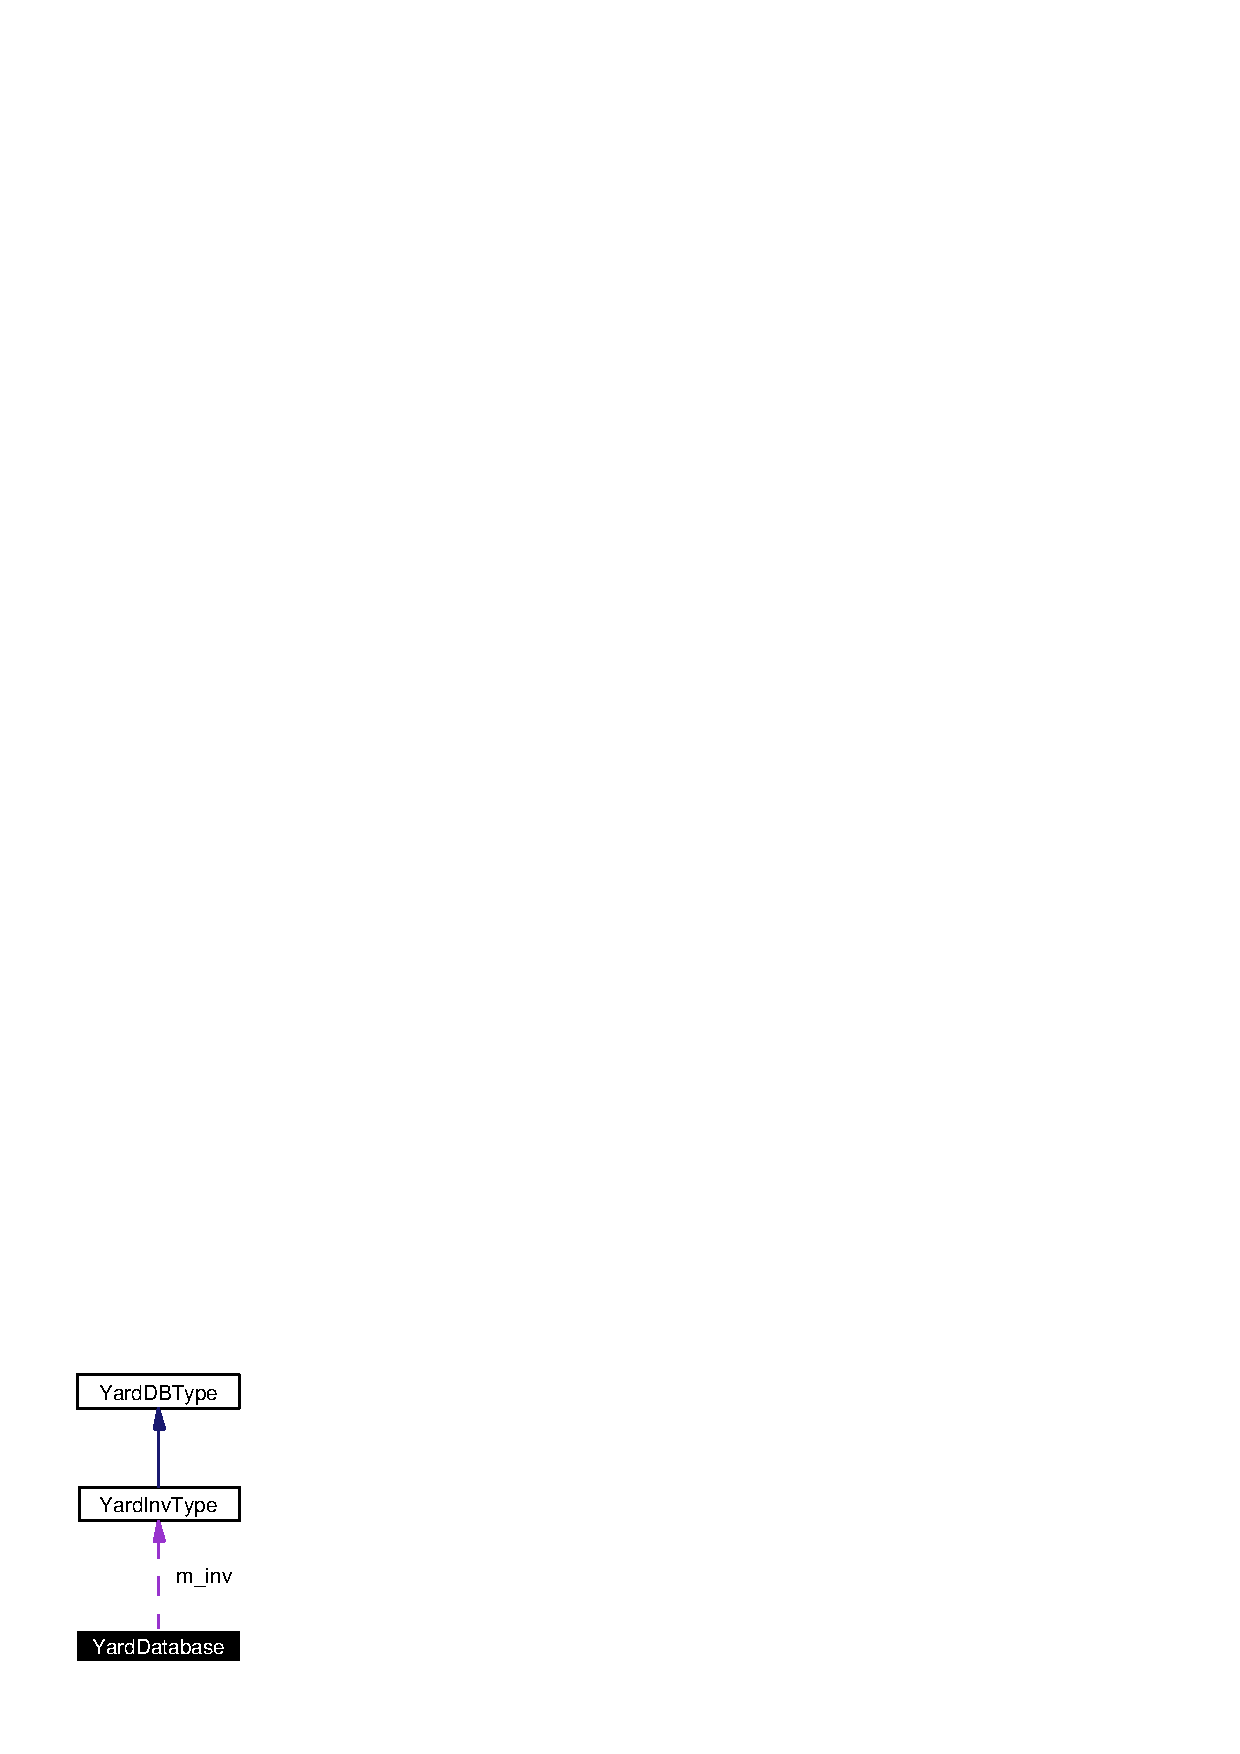
\includegraphics[width=60pt]{classYardDatabase__coll__graph}
\end{center}
\end{figure}


\subsection{Detailed Description}
This is the main database backend which does all translation from OO calls to SQL/ODBC. 

\begin{Desc}
\item[See also:]{\bf Yard\-Inv\-Type}{\rm (p.\,\pageref{classYardInvType})} \end{Desc}


\subsection*{Public Member Functions}
\begin{CompactItemize}
\item 
{\bf Yard\-Database} (const wx\-String \&dsn, const wx\-String \&name, const wx\-String \&pass)\label{classYardDatabase_a0}

\item 
bool {\bf connect} ()\label{classYardDatabase_a2}

\item 
vector$<$ {\bf Yard\-Inv\-Type} $>$ {\bf Inv\-Search\-Keyword} (const unsigned long \&sku)
\begin{CompactList}\small\item\em Find all inventory matches of keyword search. \item\end{CompactList}\item 
vector$<$ {\bf Yard\-Inv\-Type} $>$ {\bf Inv\-Get} (unsigned int num, unsigned int offset)
\begin{CompactList}\small\item\em Get a batch of inventory items. \item\end{CompactList}\end{CompactItemize}


\subsection{Member Function Documentation}
\index{YardDatabase@{Yard\-Database}!InvGet@{InvGet}}
\index{InvGet@{InvGet}!YardDatabase@{Yard\-Database}}
\subsubsection{\setlength{\rightskip}{0pt plus 5cm}vector$<${\bf Yard\-Inv\-Type}$>$ Yard\-Database::Inv\-Get (unsigned int {\em num}, unsigned int {\em offset})}\label{classYardDatabase_a4}


Get a batch of inventory items. 

\begin{Desc}
\item[Parameters:]
\begin{description}
\item[{\em num}]The number of items to get. \item[{\em offset}]The item index to start at. \end{description}
\end{Desc}
\begin{Desc}
\item[Returns:]A std::vector of {\bf Yard\-Inv\-Type}{\rm (p.\,\pageref{classYardInvType})} objects \end{Desc}
\index{YardDatabase@{Yard\-Database}!InvSearchKeyword@{InvSearchKeyword}}
\index{InvSearchKeyword@{InvSearchKeyword}!YardDatabase@{Yard\-Database}}
\subsubsection{\setlength{\rightskip}{0pt plus 5cm}vector$<${\bf Yard\-Inv\-Type}$>$ Yard\-Database::Inv\-Search\-Keyword (const unsigned long \& {\em sku})}\label{classYardDatabase_a3}


Find all inventory matches of keyword search. 

\begin{Desc}
\item[Note:]This could be dangerous, need to limit all returns to some set value (or configured value). \end{Desc}
\begin{Desc}
\item[Parameters:]
\begin{description}
\item[{\em keyword}]A text string to search for. \end{description}
\end{Desc}
\begin{Desc}
\item[Returns:]A std::vector of {\bf Yard\-Inv\-Type}{\rm (p.\,\pageref{classYardInvType})} objects \end{Desc}


The documentation for this class was generated from the following files:\begin{CompactItemize}
\item 
ys\_\-database.h\item 
ys\_\-database.cpp\end{CompactItemize}

%\section{Yard\-DBType Class Reference}
\label{classYardDBType}\index{YardDBType@{YardDBType}}
{\tt \#include $<$ys\_\-dbtype.h$>$}

Inheritance diagram for Yard\-DBType:\begin{figure}[H]
\begin{center}
\leavevmode
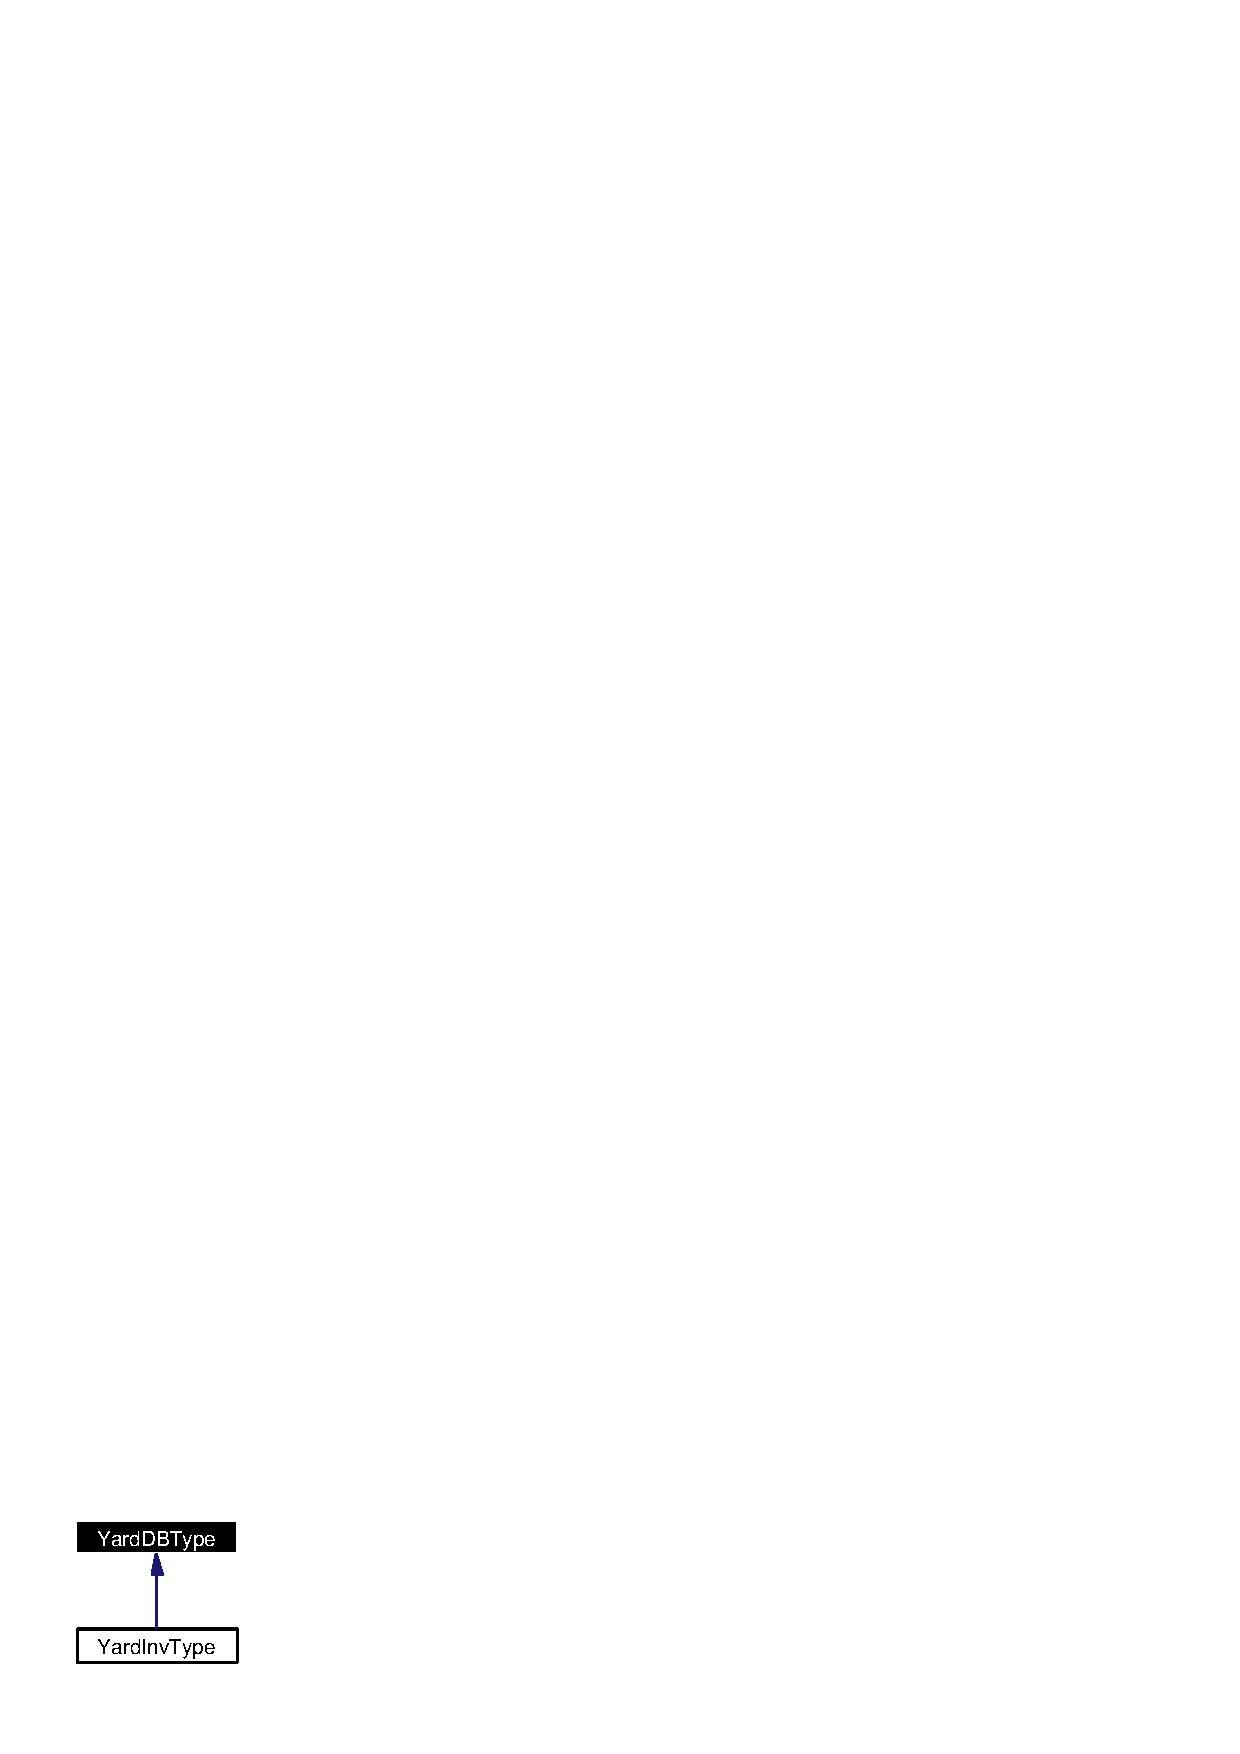
\includegraphics[width=57pt]{classYardDBType__inherit__graph}
\end{center}
\end{figure}


\subsection{Detailed Description}
Abstract base class for datebase objects in {\bf Yard\-Sale}{\rm (p.\,\pageref{classYardSale})}. 

\begin{Desc}
\item[Author:]Jesse Lovelace \end{Desc}


\subsection*{Public Member Functions}
\begin{CompactItemize}
\item 
{\bf Yard\-DBType} (const {\bf Yard\-DBType} \&obj)\label{classYardDBType_a1}

\end{CompactItemize}


The documentation for this class was generated from the following file:\begin{CompactItemize}
\item 
ys\_\-dbtype.h\end{CompactItemize}

%\section{Yard\-Employee Class Reference}
\label{classYardEmployee}\index{YardEmployee@{YardEmployee}}
{\tt \#include $<$ys\_\-employee.h$>$}



\subsection{Detailed Description}
Yard\-Employee is the employee managment screen for {\bf Yard\-Sale}{\rm (p.\,\pageref{classYardSale})}. 

Depending on access level, users may insert/modify employee information via this screen. \begin{Desc}
\item[Author:]Jesse Lovelace \end{Desc}


\subsection*{Public Member Functions}
\begin{CompactItemize}
\item 
{\bf Yard\-Employee} (wx\-Window $\ast$parent, wx\-Window\-ID id, const wx\-String \&title, const wx\-Point \&pos=wx\-Default\-Position, const wx\-Size \&size=wx\-Default\-Size, long style=wx\-RESIZE\_\-BORDER)\label{classYardEmployee_a0}

\end{CompactItemize}


The documentation for this class was generated from the following files:\begin{CompactItemize}
\item 
ys\_\-employee.h\item 
ys\_\-employee.cpp\end{CompactItemize}

%\section{Yard\-Inventory Class Reference}
\label{classYardInventory}\index{YardInventory@{YardInventory}}
{\tt \#include $<$ys\_\-inventory.h$>$}



\subsection{Detailed Description}
The inventory screen. 

\begin{Desc}
\item[Author:]Jesse Lovelace \end{Desc}
\begin{Desc}
\item[Version:]\begin{Desc}
\item[Revision]1.5 \end{Desc}
\end{Desc}


\subsection*{Public Member Functions}
\begin{CompactItemize}
\item 
{\bf Yard\-Inventory} (wx\-Window $\ast$parent, wx\-Window\-ID id, const wx\-String \&title, const wx\-Point \&pos=wx\-Default\-Position, const wx\-Size \&size=wx\-Default\-Size, long style=wx\-RESIZE\_\-BORDER)\label{classYardInventory_a0}

\item 
void {\bf On\-Exit\-Button} (wx\-Command\-Event \&event)
\begin{CompactList}\small\item\em Exit button handler. \item\end{CompactList}\end{CompactItemize}


\subsection{Member Function Documentation}
\index{YardInventory@{Yard\-Inventory}!OnExitButton@{OnExitButton}}
\index{OnExitButton@{OnExitButton}!YardInventory@{Yard\-Inventory}}
\subsubsection{\setlength{\rightskip}{0pt plus 5cm}void Yard\-Inventory::On\-Exit\-Button (wx\-Command\-Event \& {\em event})}\label{classYardInventory_a2}


Exit button handler. 

\begin{Desc}
\item[Parameters:]
\begin{description}
\item[{\em event}]The event being passed in. \end{description}
\end{Desc}


The documentation for this class was generated from the following files:\begin{CompactItemize}
\item 
ys\_\-inventory.h\item 
ys\_\-inventory.cpp\end{CompactItemize}

%\section{Yard\-Inv\-Type Class Reference}
\label{classYardInvType}\index{YardInvType@{YardInvType}}
{\tt \#include $<$ys\_\-inv\_\-type.h$>$}

Inheritance diagram for Yard\-Inv\-Type:\begin{figure}[H]
\begin{center}
\leavevmode
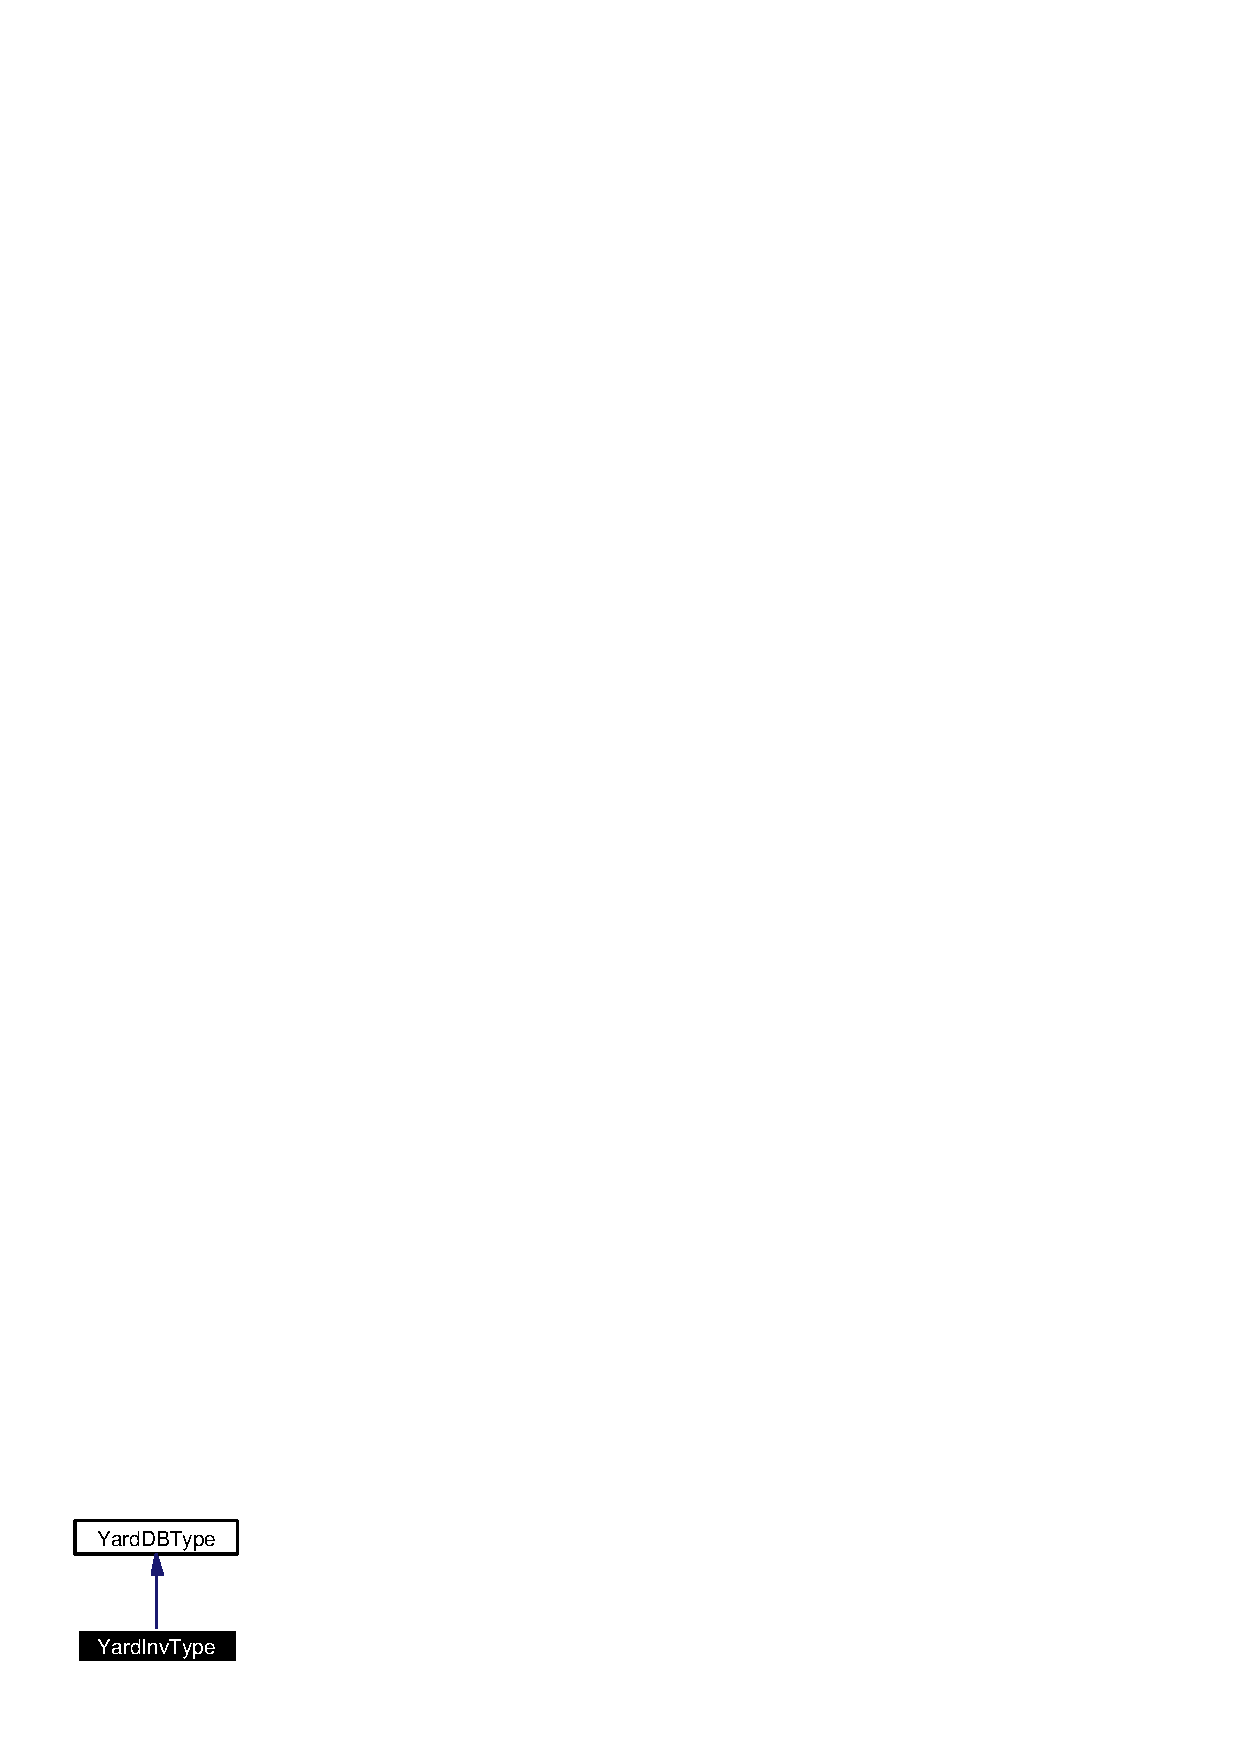
\includegraphics[width=57pt]{classYardInvType__inherit__graph}
\end{center}
\end{figure}
Collaboration diagram for Yard\-Inv\-Type:\begin{figure}[H]
\begin{center}
\leavevmode
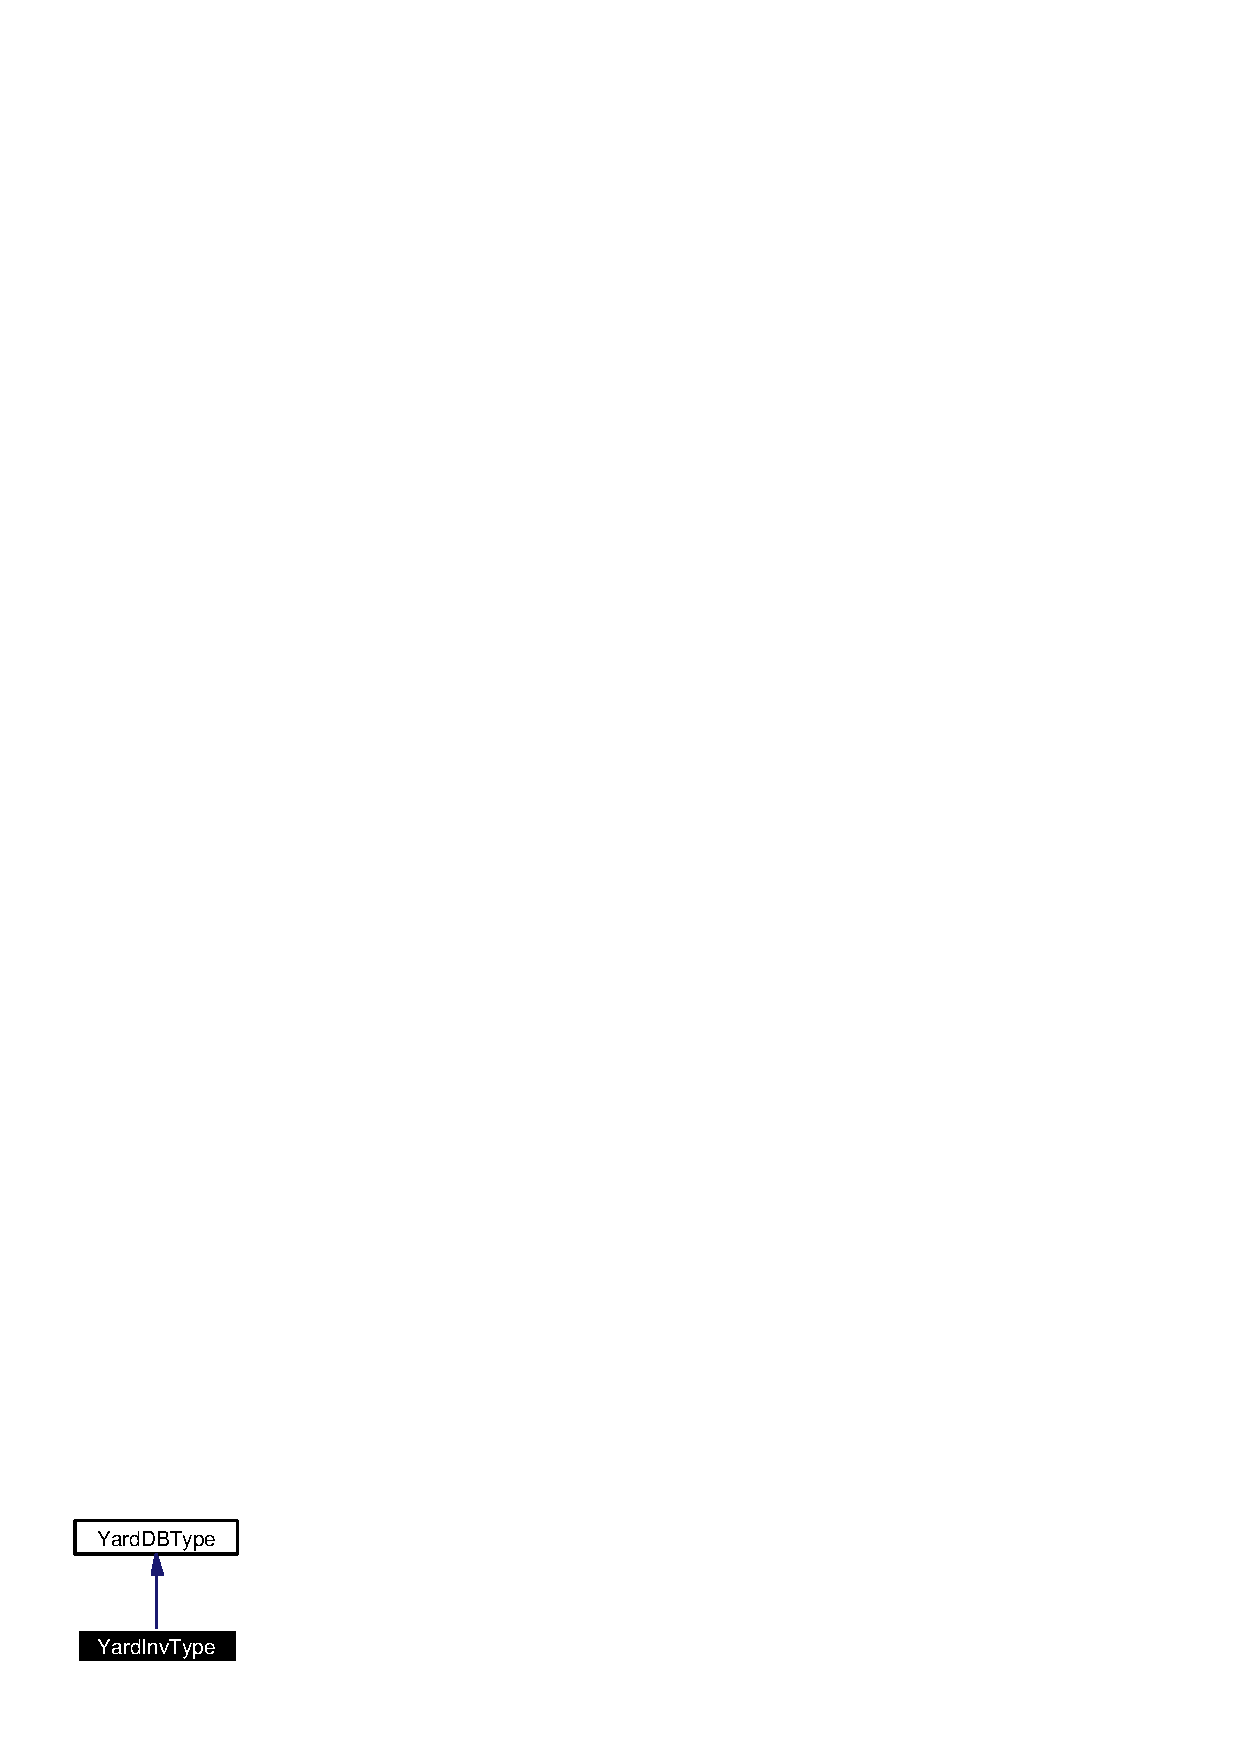
\includegraphics[width=57pt]{classYardInvType__coll__graph}
\end{center}
\end{figure}


\subsection{Detailed Description}
The {\bf Yard\-Sale}{\rm (p.\,\pageref{classYardSale})} Inventory Type is a OO representation of the datebase inventory table. 

\begin{Desc}
\item[Author:]Jesse Lovelace \end{Desc}
\begin{Desc}
\item[Version:]\begin{Desc}
\item[Revision]1.3 \end{Desc}
\end{Desc}
\begin{Desc}
\item[See also:]{\bf Yard\-DBType}{\rm (p.\,\pageref{classYardDBType})} \end{Desc}


\subsection*{Public Member Functions}
\begin{CompactItemize}
\item 
{\bf Yard\-Inv\-Type} (const {\bf Yard\-Inv\-Type} \&obj)\label{classYardInvType_a1}

\begin{CompactList}\small\item\em Copy constructor. \item\end{CompactList}\item 
{\bf Yard\-Inv\-Type} \& {\bf operator=} (const {\bf Yard\-Inv\-Type} \&obj)\label{classYardInvType_a2}

\item 
wx\-String {\bf Get\-Bar\-Code} () const \label{classYardInvType_a3}

\item 
wx\-String {\bf Get\-Description} () const \label{classYardInvType_a4}

\item 
wx\-String {\bf Get\-Department} () const \label{classYardInvType_a5}

\item 
unsigned long {\bf Get\-Quant\-On\-Hand} () const \label{classYardInvType_a6}

\item 
unsigned long {\bf Get\-Quant\-On\-Order} () const \label{classYardInvType_a7}

\item 
unsigned long {\bf Get\-Reorder\-Level} () const \label{classYardInvType_a8}

\item 
wx\-String {\bf Get\-Item\-Type} () const \label{classYardInvType_a9}

\item 
float {\bf Get\-Item\-Weight\-Lbs} () const \label{classYardInvType_a10}

\item 
float {\bf Get\-Tax\-Type} () const \label{classYardInvType_a11}

\item 
long int {\bf Get\-Vendor\-Id} () const \label{classYardInvType_a12}

\item 
float {\bf Get\-Retail\-Price} () const \label{classYardInvType_a13}

\item 
float {\bf Get\-Wholesale\-Price} () const \label{classYardInvType_a14}

\item 
vector$<$ Bulk\-Pricing $>$ {\bf Get\-Bulk\-Pricing} () const \label{classYardInvType_a15}

\item 
bool {\bf Is\-Over\-Sized} () const \label{classYardInvType_a16}

\item 
bool {\bf Must\-Ship\-Freight} () const \label{classYardInvType_a17}

\item 
void {\bf Set\-Bar\-Code} (const wx\-String \&str)\label{classYardInvType_a18}

\item 
void {\bf Set\-Description} (const wx\-String \&str)\label{classYardInvType_a19}

\item 
void {\bf Set\-Department} (const wx\-String \&str)\label{classYardInvType_a20}

\item 
void {\bf Set\-Quant\-On\-Hand} (unsigned long num)\label{classYardInvType_a21}

\item 
void {\bf Set\-Quant\-On\-Order} (unsigned long num)\label{classYardInvType_a22}

\item 
void {\bf Set\-Reorder\-Level} (unsigned long num)\label{classYardInvType_a23}

\item 
void {\bf Set\-Item\-Type} (const wx\-String \&str)\label{classYardInvType_a24}

\item 
void {\bf Set\-Item\-Weight\-Lbs} (float num)\label{classYardInvType_a25}

\item 
void {\bf Set\-Tax\-Type} (float num)\label{classYardInvType_a26}

\item 
void {\bf Set\-Ventor\-Id} (long int num)\label{classYardInvType_a27}

\item 
void {\bf Set\-Retail\-Price} (float num)\label{classYardInvType_a28}

\item 
void {\bf Set\-Wholesale\-Price} (float num)\label{classYardInvType_a29}

\item 
bool {\bf Add\-Bulk\-Price} (const Bulk\-Pricing \&price)\label{classYardInvType_a30}

\item 
bool {\bf Remove\-Bulk\-Price} (unsigned int level)\label{classYardInvType_a31}

\item 
void {\bf Set\-Over\-Sized} (bool cond)\label{classYardInvType_a32}

\item 
void {\bf Set\-Ship\-Freight} (bool cond)\label{classYardInvType_a33}

\end{CompactItemize}
\subsection*{Friends}
\begin{CompactItemize}
\item 
class {\bf Yard\-Database}\label{classYardInvType_n0}

\end{CompactItemize}


The documentation for this class was generated from the following files:\begin{CompactItemize}
\item 
ys\_\-inv\_\-type.h\item 
ys\_\-inv\_\-type.cpp\end{CompactItemize}

%\section{Yard\-Login Class Reference}
\label{classYardLogin}\index{YardLogin@{YardLogin}}
{\tt \#include $<$ys\_\-login.h$>$}



\subsection{Detailed Description}
This is the customized login screen for {\bf Yard\-Sale}{\rm (p.\,\pageref{classYardSale})}. 

\begin{Desc}
\item[Author:]Jesse Lovelace \end{Desc}
\begin{Desc}
\item[Version:]\begin{Desc}
\item[Revision]1.3 \end{Desc}
\end{Desc}


\subsection*{Public Member Functions}
\begin{CompactItemize}
\item 
{\bf Yard\-Login} (wx\-Window $\ast$parent, wx\-Window\-ID id, const wx\-String \&title, const wx\-Point \&pos=wx\-Default\-Position, const wx\-Size \&size=wx\-Default\-Size, long style=wx\-STAY\_\-ON\_\-TOP$|$wx\-RESIZE\_\-BORDER)\label{classYardLogin_a0}

\item 
void {\bf On\-Exit\-Button} (wx\-Command\-Event \&event)
\begin{CompactList}\small\item\em Exit button handler. \item\end{CompactList}\item 
void {\bf On\-Login} (wx\-Command\-Event \&event)\label{classYardLogin_a3}

\end{CompactItemize}


\subsection{Member Function Documentation}
\index{YardLogin@{Yard\-Login}!OnExitButton@{OnExitButton}}
\index{OnExitButton@{OnExitButton}!YardLogin@{Yard\-Login}}
\subsubsection{\setlength{\rightskip}{0pt plus 5cm}void Yard\-Login::On\-Exit\-Button (wx\-Command\-Event \& {\em event})}\label{classYardLogin_a2}


Exit button handler. 

\begin{Desc}
\item[Parameters:]
\begin{description}
\item[{\em event}]The event being passed in. \end{description}
\end{Desc}


The documentation for this class was generated from the following files:\begin{CompactItemize}
\item 
ys\_\-login.h\item 
ys\_\-login.cpp\end{CompactItemize}

%\section{Yard\-Main Class Reference}
\label{classYardMain}\index{YardMain@{YardMain}}
{\tt \#include $<$ys\_\-main.h$>$}



\subsection{Detailed Description}
Yard\-Main is the main menu screen for {\bf Yard\-Sale}{\rm (p.\,\pageref{classYardSale})}, it displays graphical buttons for accessing the inventory, employees, sales, etc. 

\begin{Desc}
\item[Author:]Jesse Lovelace \end{Desc}
\begin{Desc}
\item[Version:]\begin{Desc}
\item[Revision]1.6 \end{Desc}
\end{Desc}


\subsection*{Public Member Functions}
\begin{CompactItemize}
\item 
{\bf Yard\-Main} (wx\-Window $\ast$parent, wx\-Window\-ID id, const wx\-String \&title, const wx\-Point \&pos=wx\-Default\-Position, const wx\-Size \&size=wx\-Default\-Size, long style=wx\-RESIZE\_\-BORDER$|$wx\-FRAME\_\-NO\_\-TASKBAR)
\begin{CompactList}\small\item\em Constructor. \item\end{CompactList}\item 
void {\bf On\-Logout} (wx\-Command\-Event \&event)\label{classYardMain_a2}

\begin{CompactList}\small\item\em Logout button event handler. \item\end{CompactList}\item 
void {\bf On\-Max} (wx\-Command\-Event \&event)\label{classYardMain_a3}

\begin{CompactList}\small\item\em Maximize handler. \item\end{CompactList}\item 
void {\bf On\-Inventory} (wx\-Command\-Event \&event)\label{classYardMain_a4}

\begin{CompactList}\small\item\em Inventory button handler. \item\end{CompactList}\item 
void {\bf On\-Sale} (wx\-Command\-Event \&event)\label{classYardMain_a5}

\begin{CompactList}\small\item\em Sales buttons. \item\end{CompactList}\item 
void {\bf On\-Employee} (wx\-Command\-Event \&event)\label{classYardMain_a6}

\begin{CompactList}\small\item\em Employee button handler. \item\end{CompactList}\end{CompactItemize}


\subsection{Constructor \& Destructor Documentation}
\index{YardMain@{Yard\-Main}!YardMain@{YardMain}}
\index{YardMain@{YardMain}!YardMain@{Yard\-Main}}
\subsubsection{\setlength{\rightskip}{0pt plus 5cm}Yard\-Main::Yard\-Main (wx\-Window $\ast$ {\em parent}, wx\-Window\-ID {\em id}, const wx\-String \& {\em title}, const wx\-Point \& {\em pos} = wx\-Default\-Position, const wx\-Size \& {\em size} = wx\-Default\-Size, long {\em style} = wx\-RESIZE\_\-BORDER$|$wx\-FRAME\_\-NO\_\-TASKBAR)}\label{classYardMain_a0}


Constructor. 



\begin{Desc}
\item[{\bf Todo}]Make these compiled into the binary.\end{Desc}


The documentation for this class was generated from the following files:\begin{CompactItemize}
\item 
ys\_\-main.h\item 
ys\_\-main.cpp\end{CompactItemize}

%\section{Yard\-Sale Class Reference}
\label{classYardSale}\index{YardSale@{YardSale}}
{\tt \#include $<$yardsale.h$>$}



\subsection{Detailed Description}
This is the main application object. 

\begin{Desc}
\item[Author:]Jesse Lovelace \end{Desc}
\begin{Desc}
\item[Version:]\begin{Desc}
\item[Revision]1.8 \end{Desc}
\end{Desc}


\subsection*{Public Member Functions}
\begin{CompactItemize}
\item 
virtual bool {\bf On\-Init} ()
\begin{CompactList}\small\item\em This is the function were top level windows are created. \item\end{CompactList}\end{CompactItemize}


\subsection{Member Function Documentation}
\index{YardSale@{Yard\-Sale}!OnInit@{OnInit}}
\index{OnInit@{OnInit}!YardSale@{Yard\-Sale}}
\subsubsection{\setlength{\rightskip}{0pt plus 5cm}bool Yard\-Sale::On\-Init ()\hspace{0.3cm}{\tt  [virtual]}}\label{classYardSale_a0}


This is the function were top level windows are created. 

\begin{Desc}
\item[Returns:]True if application initialized ok \end{Desc}


The documentation for this class was generated from the following files:\begin{CompactItemize}
\item 
yardsale.h\item 
yardsale.cpp\end{CompactItemize}

%\section{Yard\-Sale\-Screen Class Reference}
\label{classYardSaleScreen}\index{YardSaleScreen@{YardSaleScreen}}
{\tt \#include $<$ys\_\-sale.h$>$}



\subsection{Detailed Description}
This is the main sale screen. 

It contains the current transaction information. \begin{Desc}
\item[Author:]Jesse Lovelace \end{Desc}
\begin{Desc}
\item[Version:]\begin{Desc}
\item[Revision]1.3 \end{Desc}
\end{Desc}


\subsection*{Public Member Functions}
\begin{CompactItemize}
\item 
{\bf Yard\-Sale\-Screen} (wx\-Window $\ast$parent, wx\-Window\-ID id, const wx\-String \&title, const wx\-Point \&pos=wx\-Default\-Position, const wx\-Size \&size=wx\-Default\-Size, long style=wx\-RESIZE\_\-BORDER)\label{classYardSaleScreen_a0}

\item 
void {\bf On\-Exit\-Button} (wx\-Command\-Event \&event)\label{classYardSaleScreen_a2}

\begin{CompactList}\small\item\em Exit button event handler. \item\end{CompactList}\end{CompactItemize}


The documentation for this class was generated from the following files:\begin{CompactItemize}
\item 
ys\_\-sale.h\item 
ys\_\-sale.cpp\end{CompactItemize}

%\section{Yard\-Splash Class Reference}
\label{classYardSplash}\index{YardSplash@{YardSplash}}
{\tt \#include $<$ys\_\-splash.h$>$}



\subsection{Detailed Description}
Eye-candy splash screen. 

\begin{Desc}
\item[Author:]Jesse Lovelace \end{Desc}
\begin{Desc}
\item[Version:]\begin{Desc}
\item[Revision]1.6 \end{Desc}
\end{Desc}


\subsection*{Public Member Functions}
\begin{CompactItemize}
\item 
{\bf Yard\-Splash} (wx\-Window $\ast$parent, wx\-Window\-ID id, const wx\-String \&title, const wx\-Point \&pos=wx\-Default\-Position, const wx\-Size \&size=wx\-Default\-Size, long style=wx\-STAY\_\-ON\_\-TOP)\label{classYardSplash_a0}

\item 
void {\bf On\-Click} (wx\-Mouse\-Event \&event)
\begin{CompactList}\small\item\em Mouse click event handler. \item\end{CompactList}\item 
void {\bf On\-Timer} (wx\-Timer\-Event \&event)\label{classYardSplash_a3}

\begin{CompactList}\small\item\em Timer event handler. \item\end{CompactList}\item 
void {\bf Bump} (unsigned int amount=10)
\begin{CompactList}\small\item\em Called to nudge progress bar over. \item\end{CompactList}\end{CompactItemize}


\subsection{Member Function Documentation}
\index{YardSplash@{Yard\-Splash}!Bump@{Bump}}
\index{Bump@{Bump}!YardSplash@{Yard\-Splash}}
\subsubsection{\setlength{\rightskip}{0pt plus 5cm}void Yard\-Splash::Bump (unsigned int {\em amount} = 10)}\label{classYardSplash_a4}


Called to nudge progress bar over. 

\begin{Desc}
\item[Parameters:]
\begin{description}
\item[{\em amount}]Number of pixels to nudge \end{description}
\end{Desc}
\index{YardSplash@{Yard\-Splash}!OnClick@{OnClick}}
\index{OnClick@{OnClick}!YardSplash@{Yard\-Splash}}
\subsubsection{\setlength{\rightskip}{0pt plus 5cm}void Yard\-Splash::On\-Click (wx\-Mouse\-Event \& {\em event})}\label{classYardSplash_a2}


Mouse click event handler. 

\begin{Desc}
\item[{\bf Deprecated}]This handler is for testing only and will be removed \end{Desc}


The documentation for this class was generated from the following files:\begin{CompactItemize}
\item 
ys\_\-splash.h\item 
ys\_\-splash.cpp\end{CompactItemize}


\chapter{Test Plan}

\end{document}
